\documentclass[table, 12pt]{article}
\usepackage[a4paper, top=25mm, bottom=25mm, left=20mm, right=20mm]{geometry}
\usepackage{graphicx}
\usepackage[T1]{fontenc}
\usepackage[default]{cantarell}
\usepackage{tocloft}
\usepackage{caption}
\usepackage{minted}
\usepackage{hyperref}
\usepackage{booktabs}
\usepackage{listings}
\usepackage{pdfpages}
\usepackage{pdflscape}
\usepackage{textpos}
\usepackage{scrhack}
\usepackage{xcolor}
\usepackage{mathptmx}
\usepackage{float}
\usepackage{longtable}
\usepackage{enumitem}
\usepackage{tasks}
\usepackage{tabularx}
\usepackage{titlesec}
\usepackage{graphicx}
\usepackage {float}

\newcommand{\red}{\color{red}}

\titleformat{\paragraph}
{\normalfont\normalsize\bfseries}{\theparagraph}{1em}{}
\titlespacing*{\paragraph}
{0pt}{3.95ex plus 1ex minus .2ex}{.5ex plus .2ex}

\begin{document}
\begin{titlepage}
    \centering
    \vspace{2cm}
    \scshape\large Academic Year 2020/2021 \par
    \vfill
    
\includegraphics[width=200pt]{images/LogoPoliMI}\par\vspace{1cm}
    {\scshape\LARGE Computer Science and Engineering \par}
    \vspace{1.5cm}
    {\Large\bfseries System and Methods for Big and Unstructured Data \par}
    \vspace{0.5cm}
    {\huge\bfseries \textbf{Project Report - Neo4j} \par}
    \vspace{2cm}
    {\large{Matteo Falzi \quad Fabio La Manna \quad Filippo Manzardo \\Paolo Marzolo \quad Matteo Regge}\par}
    \vfill
    {\large Prof. Marco Brambilla }
    \vfill
    {\large \textbf{Version 0.1}\\ \today \par}
\end{titlepage}
\hypersetup{%
    pdfborder = {0 0 0}
}
\thispagestyle{plain}
\pagenumbering{gobble}
\mbox{}

%%%%%%%%%%%%%%%%%%%%%%%%%%%%%%%%%%%%%%%%%%%%%%%%%%%%%%%%%%%%%%%%%

\section{Introduction}

\subsection{Assumptions}
The development of application for tracing the movement of people have seen a increasing due to the Covid pandemic. The aim of these apps is to record  paths and meeting of people thus to contain the spread of the virus. The project consist of modeling an app, that uses a NoSQL DB, for that purpose.

\subsection{Delivery specification}
The problem consinst in storing the movements of the user and all people that he met during the day, using Neo4j, a graph NoSQL DB. In addition we have to provide a few queries and commands. We have to discern the family group from the other people, whom are the default contact of the user.

\subsection{Hypothesis }
\begin{description}

\item[Places:]We consider the possibility for a place to have a room, moreover we always know the date and how much time the user spend in that place.
\item[Contacts:]We consider a contact between the user and another person in a specific date, we always know the duration of the meeting.We taking into consideration that two or more people can move from place to place together, in addition every time of the user changes place the app stores the information, so we don't record the information of the place in the contacts. 
\item[Personal data:]
We consider that a person may or may not  have a vaccine/test.
\end{description} 
%%%%%%%%%%%%%%%%%%%%%%%%%%%%%%%%%%%%%%%%%%%%%%%%%%%%%%%%%%%%%%%%%


\section{Relational Model}
\subsection{Logic Model}
Following the image of the ER diagram and the descriptions of the classes and relations.
\begin{center}
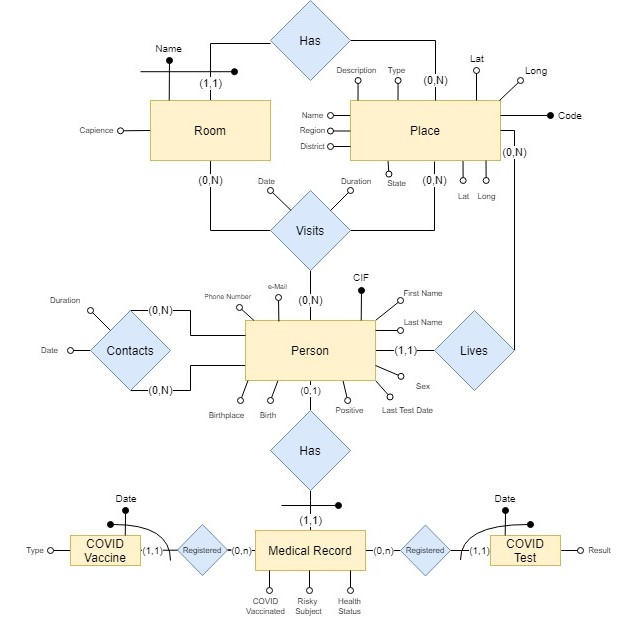
\includegraphics[width=0.65\textwidth]{images/e.jpg} 
\end{center}

\begin{minted}
    [
    frame=lines,
    framesep=5mm,
    baselinestretch=1.5,
    escapeinside=||
    ]
    {python}
    ####### Entities #######
    Person(|\red{CIF}|,Name,Surname,Birth,Sex,Birthplace,Phone_Number, e-Mail, Positive,Last_Confirm)
    Place(|\red{Code}|,Name,Lat,Long,CAP,State,Region,District,Type,Type_Desc)
    Room(|\red{code}|,Name,Capience)
    Medical_Record(|\red{CIF}|,Covid_Vaccinated,Risky_Subject,Health_Status)
    Covid_Tests(|\red{CIF}|,|\red{Date}|,Results)
    Covid_Vaccines(|\red{CIF}|,|\red{Date}|,Type)
   
    
    
    ####### Relations #######
    Has(|\red{CIF}|)
    Has(|\red{Code}|)
    Registered(|\red{CIF}|,|\red{Date}|)
    Registered(|\red{CIF}|,|\red{Date}|)
    Contacts(|\red{CIF}|,|\red{CIF}|,Date,Duration)
    Lives(|\red{CIF}|,|\red{cif}|)
    Visit(|\red{CIF}|,|\red{code}|,Date,Duration)
    
            
\end{minted}

\begin{description}
\item[Person:] contains the personal information, furthermore has the positiveness and the last confirm of it.
We use the last confirm to be able to change the value of the attribute "positive" according with the latest test, moreover if it is true there is at least one covid test in Medical record.
\item[Place:] contains the geographic information, the type and a description.
\item[Room:] contains the name and the capience of the room.
\item[Medical Record:] contains health status,the measure of risk of the user and if he is vaccinated, if it is true there is at least one covid Vaccine. Which collect,by the relations Registered all the tests and the vaccines.
\item[Covid Tests:] contains the date and the results of the covid test.
\item[Covid Vaccines:] contains the date and the type of the covid vaccine.
\item[Has(CIF)] is the relation between Person and Medical Record,can be absent or at most one.
\item[Has(Code):] is the relation between Place and Room, a place has zero or more rooms, but the room is  only of one place.
\item[Registered:] are the relations by which tests or vaccines are collected in the Medical records.
\item[Contacts:] is the relation that keeps track of the meetings and their duration in a certain date.
\item[Lives:] is the relation trough which we can identify all the components of one family. The user have to live in one place, but not all  places are inhabited.
\item[Visit:] is the relations is the relation that keeps track of all visits in Places/Rooms and their duration in a certain date.


\end{description} 

%%%%%%%%%%%%%%%%%%%%%%%%%%%%%%%%%%%%%%%%%%%%%%%%%%%%%%%%%%%%%%%%%

\section{Dataset}
The datasets are made in python, almost the totality of the data are generated with random functions.

\begin{minted}
    [
    frame=lines,
    framesep=5mm,
    baselinestretch=1.5,
    escapeinside=||
    ]
    {text}
     sex = random.choice(['male','female'])
     first_name = names.get_first_name(gender=sex)
     last_name = names.get_last_name()
     positive = random.choice([True, False], p=[positive_ratio, 1 - positive_ratio])
     birth = (birth_min_datetime + (birth_max_datetime - birth_min_datetime) 
     * random.random()).strftime('%Y-%m-%d')
     phone_number = randomPhone()
     mail_provider  = random.choice(['gmail.com','outlook.it','icloud.com',
     'hotmail.it','yahoo.it'])
     email = f'{first_name.lower()}.{last_name.lower()}@{mail_provider}'
     if positive:
        last_confirm = (min_positive_datetime + (max_datetime - min_positive_datetime) * random.random()).strftime('%Y-%m-%d')
    else:
        last_confirm = random.choice([None, (min_datetime + (max_datetime 
        - min_datetime) * random.random()).strftime('%Y-%m-%d')],
        p=[tested_ratio,1-tested_ratio])
    
    sex = sex[0].upper()
    birthplace = cities[random.randint(0,len(cities))]
    
    try:
         CIF = codicefiscale.encode(surname=last_name, name=first_name, sex=sex, birthdate=birth, birthplace=birthplace)
    people.append({
        'CIF': CIF,
        'First_Name': first_name,
        'Last_Name': last_name,
        'Positive': positive,
        'Birth': birth,
        'Birthplace': birthplace,
        'Phone_Number': phone_number,
        'Email': email,
        'Last_Confirm': last_confirm,
        'Sex': sex
        })

\end{minted}

The \textbf{\red{Person}} dataset is made: \textbf{name} and \textbf{last name} by a function of names package, \textbf{sex}/\textbf{positive} by a random choice between the two values,\textbf{phone number}/\textbf{mail}/\textbf{birth} by a random function, \textbf{last confirm} by two random function: if positive  is true the function range is from fourtyfive days before now to now else the function range is from 1/1/2020 to now,\textbf{birthplace} by extraction of a value from csv and \textbf{CIF} by a function of codicefiscale package.
%%%%%Medical Records%%%%%
\begin{minted}
    [
    frame=lines,
    framesep=5mm,
    baselinestretch=1.5,
    escapeinside=||
    ]
    {text}
        covid_vaccinated = random.choice([True, False])
        risky_subject = random.choice([True, False], p=[risky_ratio, 1 - risky_ratio])
        health_status = random.choice(["bad", "average", "good"])

        medical_records.append({
                'CIF': CIF,
                'Covid_Vaccinated': covid_vaccinated,
                'Risky_Subject': risky_subject,
                'Health_Status': health_status,
        })

\end{minted}
The \textbf{\red{Medical Records}} dataset is made: \textbf{CIF} of the current person,\textbf{risky subject}/\textbf{Covid vaccinated} by a random choice between ("true","false") and \textbf{health status} by a random choice between ("bad","average","good").
%%%%%Covid vaccines%%%%%
\begin{minted}
    [
    frame=lines,
    framesep=5mm,
    baselinestretch=1.5,
    escapeinside=||
    ]
    {text}
    if (covid_vaccinated):
                for i in range(random.randint(1,3)):
                    covid_vaccines.append({
                        'CIF': CIF,
                        'Date': (min_datetime + (max_datetime - min_datetime) * random.random()).strftime('%Y-%m-%d'),
                        'Type': random.choice(["Pfizer", "Moderna", "Astrazeneca", "Johnson & Johnson"])

\end{minted}


The \textbf{\red{Covid vaccines}} dataset is made: \textbf{CIF} of the current person,\textbf{Date} by a random function and \textbf{Type} by a random choice between ("Pfizer", "Moderna", "Astrazeneca", "Johnson e Johnson") with a restriction of at most 2 vaccines per person.

%%%%%Covid tests
\begin{minted}
    [
    frame=lines,
    framesep=5mm,
    baselinestretch=1.5,
    escapeinside=||
    ]
    {text}
        # At leats one test if last_confirm (with the same result as Person.Positive)
        if (last_confirm):
            covid_tests.append({
                'CIF': CIF,
                'Date': last_confirm,
                'Result': positive,
            })

            # Discrete ~Normal Distribution~ centered in 0 for number of test per person
            x = arange(0, max_tests)
            xU, xL = x + 0.5, x - 0.5 
            prob = ss.norm.cdf(xU, scale = 3) - ss.norm.cdf(xL, scale = 3)
            prob = prob / prob.sum() 
            num = random.choice(x, p=prob)

            for i in range(num):
                covid_tests.append({
                    'CIF': CIF,
                    'Date': (min_datetime + (datetime.strptime(last_confirm,'%Y-%m-%d') - min_datetime) * random.random()).strftime('%Y-%m-%d'),
                    'Result': random.choice([True,False], p=[positive_ratio, 1 - positive_ratio])
                })

\end{minted}

The \textbf{\red{Covid tests}} dataset is made: \textbf{CIF} of the current person,\textbf{Date} equals to last confirm of the person if it's positive and \textbf{Result} equals to "positive". This cover with at least one test positives. After which a cycle to make more tests, at most ten per person.
%%%%%Places
\begin{minted}
    [
    frame=lines,
    framesep=5mm,
    baselinestretch=1.5,
    escapeinside=||
    ]
    {text}
 
    n = len(places_df)
    idxs = zeros(n)

    # Get #NUMBER_OF_PLACES random places from bigger dataset
    for i in range (NUMBER_OF_PLACES):
      l = random.randint(0,n)
      idxs[l] = places_df['Code'][l]

    places = places_df[places_df['Code'] == idxs].to_dict('records')
    del places_df

    # Generate Rooms
    rooms = []
    current_place = {'Type': None}

    for i in range(NUMBER_OF_ROOMS):
        while not(hasRooms(current_place['Type'])):
            current_place = places[random.randint(0,len(places))]

        room_name = randomRoomName()
        capience = random.randint(0, max_capience)
        rooms.append({
                'Code': current_place['Code'],
                'Name': room_name,
                'Capience': capience
            })
        current_place = {'Type': None}
\end{minted}
The \textbf{\red{Places }} dataset is made: \textbf{Code} by a key generator function, and the other values by a csv o places, \textbf{type} by a random function.
%%%%%Rooms
The \textbf{\red{Rooms }} dataset is made: \textbf{room name } by a custom function,  \textbf{capience} by a random function with max set to 150, \textbf{code} by a key generator function.
%%%%%Contacts
\begin{minted}
    [
    frame=lines,
    framesep=5mm,
    baselinestretch=1.5,
    escapeinside=||
    ]
    {text}
def getRelations(people, places, rooms):

    contacts = []
    visits =  []
    lives = []

    # Generate Contacts
    for i in range(NUMBER_OF_CONTACTS):

        contact_date = (min_datetime + (max_datetime - min_datetime) * random.random()).strftime('%Y-%m-%d')
        time = timedelta(minutes=random.randint(min_contact_duration, max_contact_duration))
        contact_duration = '{:02.0f}:{:02.0f}:00'.format(floor(time.seconds/3600), time.seconds % 3600 /60)

        P1 = random.randint(0, NUMBER_OF_PEOPLE) 
        P2 = random.randint(0, NUMBER_OF_PEOPLE)

        # No contact with itself
        if P1 == P2:
            P2 -= 1

        contacts.append(
            {
                'CIF1': people[P1]['CIF'],
                'CIF2': people[P2]['CIF'],
                'Date': contact_date,
                'Duration': contact_duration
            })
\end{minted}
The \textbf{\red{Contacts }} dataset is made: \textbf{CIF1}/\textbf{CIF2} by taking two random people,\textbf{Date} by random function and \textbf{Duration} by a random function with range from 10 minutes to 1439 minutes.
%%%%%Visits
\begin{minted}
    [
    frame=lines,
    framesep=5mm,
    baselinestretch=1.5,
    escapeinside=||
    ]
    {text}
    # Generate Visits
    for i in range(NUMBER_OF_VISITS):

        visit_date = (min_datetime + (max_datetime - min_datetime) * random.random()).strftime('%Y-%m-%d')
        time = timedelta(minutes=random.randint(min_contact_duration, max_contact_duration))
        visit_duration = '{:02.0f}:{:02.0f}:00'.format(floor(time.seconds/3600), time.seconds % 3600 /60)

        person = random.randint(0, NUMBER_OF_PEOPLE - 1)
        room = random.choice([None, random.randint(0, NUMBER_OF_ROOMS)])

        # If the place has no Rooms
        if room is None:
            place = places[random.randint(0, NUMBER_OF_PLACES)]
            while hasRooms(place['Type']):
                place = places[random.randint(0, NUMBER_OF_PLACES)]

            visits.append(
            {
                'CIF': people[person]['CIF'],
                'Place': place['Code'],
                'Room': None,
                'Date': visit_date,
                'Duration': visit_duration

            })

        else:
            visits.append(
            {
                'CIF': people[person]['CIF'],
                'Place': rooms[room]['Code'],
                'Room': rooms[room]['Name'],
                'Date': visit_date,
                'Duration': visit_duration
            })
\end{minted}
The \textbf{\red{Visits }} dataset is made: \textbf{CIF1} by taking one random person,\textbf{Place}, by taking the code of one random place,\textbf{Room} is equals to "none" if the place type don't has a room else by taking a random room ,\textbf{Date} by random function and \textbf{Duration} by a random function with range from 5 minutes to 720 minutes.
%%%%%Lives
\begin{minted}
    [
    frame=lines,
    framesep=5mm,
    baselinestretch=1.5,
    escapeinside=||
    ]
    {text}
        # Generate Lives
    people_copy = people.copy()
    random.shuffle(people_copy)

    while(len(people_copy) > 0):

        number_of_familiars = random.randint(0,6)
        if number_of_familiars >= len(people_copy):
            number_of_familiars = len(people_copy) -1

        comb = list(combinations(range(number_of_familiars), 2))
        for i in range(0,len(comb)):
            p1, p2 = comb[i]
            lives.append(
            {
                'CIF1': people_copy[p1]['CIF'],
                'CIF2': people_copy[p2]['CIF'],
            })
        people_copy = people_copy[number_of_familiars + 1:]


\end{minted}
The \textbf{\red{Lives }} dataset is made: dataset is made: taking one person and link together al least one and at most 6 people

%%%%%%%%%%%%%%%%%%%%%%%%%%%%%%%%%%%%%%%%%%%%%%%%%%%%%%%%%%%%%%%%%

\section{Neo4j Implementation}

\subsection{Queries}
\begin{minted}
    [ escapeinside=||]
    {text}
 ## ADD PEOPLE 
LOAD CSV WITH HEADERS FROM "file:///people.csv" as CSV 
CREATE(p:Person{CIF: CSV.CIF, First_Name: CSV.First_Name, Last_Name: CSV.Last_Name, 
Birth: CSV.Birth, Sex: CSV.Sex, Birthplace: CSV.Birthplace, Phone_Number:
CSV.Phone_Number, eMail: CSV.Email, Positive: toBoolean(CSV.Positive), 
Last_Confirm: Date(CSV.Last_Confirm)})

## ADD PLACES 
LOAD CSV WITH HEADERS FROM "file:///places.csv" as CSV 
CREATE(p:Place{Code: ToInteger(CSV.Code), Name: CSV.Name, Lat: ToFloat(CSV.Lat), 
Long: ToFloat(CSV.Long), CAP: ToInteger(CSV.CAP), State: CSV.State, 
Region: CSV.Region, District: CSV.District, Type: CSV.Type, Type_Desc: CSV.Type_Desc})

## ADD MEDICAL RECORDS PLUS RELATION WITH PERSON 
LOAD CSV WITH HEADERS FROM "file:///medical_records.csv" as CSV 
MATCH(p:Person{CIF: CSV.CIF})
MERGE(m:Medical_Record{CIF: p.CIF, Covid_Vaccinated: toBoolean(CSV.Covid_Vaccinated), 
Risky_Subject: toBoolean(CSV.Risky_Subject), Health_Status: CSV.Health_Status})
create(p)-[:HAS]->(m)

## ADD COVID VACCINES PLUS RELATION WITH MEDICAL RECORD 
LOAD CSV WITH HEADERS FROM "file:///covid_vaccines.csv" as CSV 
MATCH(m:Medical_Record{CIF: CSV.CIF})
MERGE(v:Covid_Vaccines{CIF: m.CIF, Date: Date(CSV.Date), Type: CSV.Type})
CREATE(m)-[:REGISTERED]->(v)

## ADD COVID TEST PLUS RELATION WITH MEDICAL RECORD 
LOAD CSV WITH HEADERS FROM "file:///covid_tests.csv" as CSV 
MATCH(m:Medical_Record{CIF: CSV.CIF})
MERGE(t:Covid_Tests{CIF: m.CIF, Date: Date(CSV.Date), Result: toBoolean(CSV.Result)})
CREATE(m)-[:REGISTERED]->(t)

## ADD ROOMS PLUS RELATION WITH PLACE
LOAD CSV WITH HEADERS FROM "file:///rooms.csv" as CSV 
MATCH(p:Place{Code: ToInteger(CSV.Code)})
MERGE(r:Rooms{Code: ToInteger(p.Code), Name: CSV.Name, 
Capience: ToInteger(CSV.Capience)})
CREATE(p)-[:HAS]->(r)

## ADD BOTH CONTACTS 
LOAD CSV WITH HEADERS FROM "file:///contacts.csv" as CSV 
MATCH(p1:Person{CIF: CSV.CIF1}),(p2:Person{CIF: CSV.CIF2}) 
MERGE(p1)-[:CONTACTS{Date: Date(CSV.Date), Duration: Time(CSV.Duration)}]->(p2)
MERGE(p2)-[:CONTACTS{Date: Date(CSV.Date), Duration: Time(CSV.Duration)}]->(p1)


## ADD LIVES RELATION
LOAD CSV WITH HEADERS FROM "file:///lives.csv" as CSV
MATCH(p1:Person{CIF: CSV.CIF1}), (p2:Person{CIF: CSV.CIF2})
MERGE (p1)-[:LIVES]-(p2)

## ADD VISIT RELATION WITH ROOM
LOAD CSV WITH HEADERS FROM "file:///visits.csv" as CSV with CSV where CSV.Room
is not null
MATCH(p:Person{CIF: CSV.CIF}),(r:Rooms{Code: ToInteger(CSV.Place), Name: CSV.Room}) 
MERGE(p)-[v:VISITS{Date: Date(CSV.Date), Duration: Time(CSV.Duration)}]->(r)

## ADD VISIT WITHOUT ROOM
LOAD CSV WITH HEADERS FROM "file:///visits.csv" as CSV with CSV where CSV.Room is null
MATCH(p:Person{CIF: CSV.CIF}),(pl:Place{Code: ToInteger(CSV.Place)}) 
MERGE(p)-[v:VISITS{Date: Date(CSV.Date), Duration: Time(CSV.Duration)}]->(pl)

\end{minted}

\subsection{Queries}
\begin{minted}
    [ escapeinside=||]
    {text}
##If a person has done at least 1 vaccine, set his Vaccinated attribute to true
match (p:Person)-[:HAS]->(m:Medical_Record), (m)-[:REGISTERED]->(v:Covid_Vaccines) 
set m.Vaccinated=True
return distinct m, v


##If a person results negative in his latest test then set is Positive attribute to false
match (p:Person)-[:HAS]->(m:Medical_Record), (m)-[:REGISTERED]->(t:Covid_Tests)
with p, max(t.Date) as Max_Date
match(p)-[:HAS]->(m:Medical_Record), (m)-[:REGISTERED]->(t:Covid_Tests)
where t.Date = Max_Date and t.Result=False
set p.Positive = False
return p, m, t


##Delete all rooms never visited from any person  
match (p:Person), (r:Room)
where not exists ((p)-[:VISITS]->(r))
detach delete r


##Delete all people without medical record
match (p:Person)
where not (p)-[:HAS]->(:Medical_Record)
detach delete p
\end{minted}
%%%%%%%%%%%%%%%%%%%%%%%%%%%%%%%%%%%%%%%%%%%%%%%%%%%%%%%%%%%%%%%%%

\section{User Interface Implementation}

%%%%%%%%%%%%%%%%%%%%%%%%%%%%%%%%%%%%%%%%%%%%%%%%%%%%%%%%%%%%%%%%%

\section{Conclusion}

:)
\end{document}
